The default settings for the experiments run in this research are shown in table \ref{tab:default}.

\begin{table}[H]
\begin{tabular}{|l|l|}
\hline
\textbf{Parameter} & \textbf{Default value}\\
\hline
Color space & Opponent\\
SIFT type & Dense\\
Training set size feature histogram & 75 per class\\
Training set size SVM & 75 per class\\
Test set size & 50 per class \\
Cluster size & 400 \\
Step size (only for dense SIFT) & 20\\
\hline
\end{tabular}
\caption{Default values for experiments}
\label{tab:default}
\end{table}

\subsection{Effect of different color spaces in key-point SIFT}

\begin{table}[H]
\begin{tabular}{|c|ccccc|}
\hline
\textbf{Color space} & \textbf{AP Airplanes} & \textbf{AP Cars} & \textbf{AP Faces} & \textbf{AP Motorbikes} & \textbf{MAP}\\
\hline
gray & & & & & \\
normalizedRGB & & & & & \\
RGB & & & & & \\
opponent & & & & & \\
\hline
\end{tabular}
\caption{Effect of different color spaces for key SIFT}
\end{table}


\subsection{Effect of different color spaces in dense SIFT}

\begin{table}[H]
\begin{tabular}{|c|ccccc|}
\hline
\textbf{Color space} & \textbf{AP Airplanes} & \textbf{AP Cars} & \textbf{AP Faces} & \textbf{AP Motorbikes} & \textbf{MAP}\\
\hline
gray & & & & & \\
normalizedRGB & & & & & \\
RGB & & & & & \\
opponent & 0.6447 & 0.9053 & 0.9510 & 0.7516 & 0.8132\\
\hline
\end{tabular}
\caption{Effect of different color spaces for dense SIFT}
\end{table}



\subsection{Effect number of training samples for feature histogram}
\begin{figure}[H]
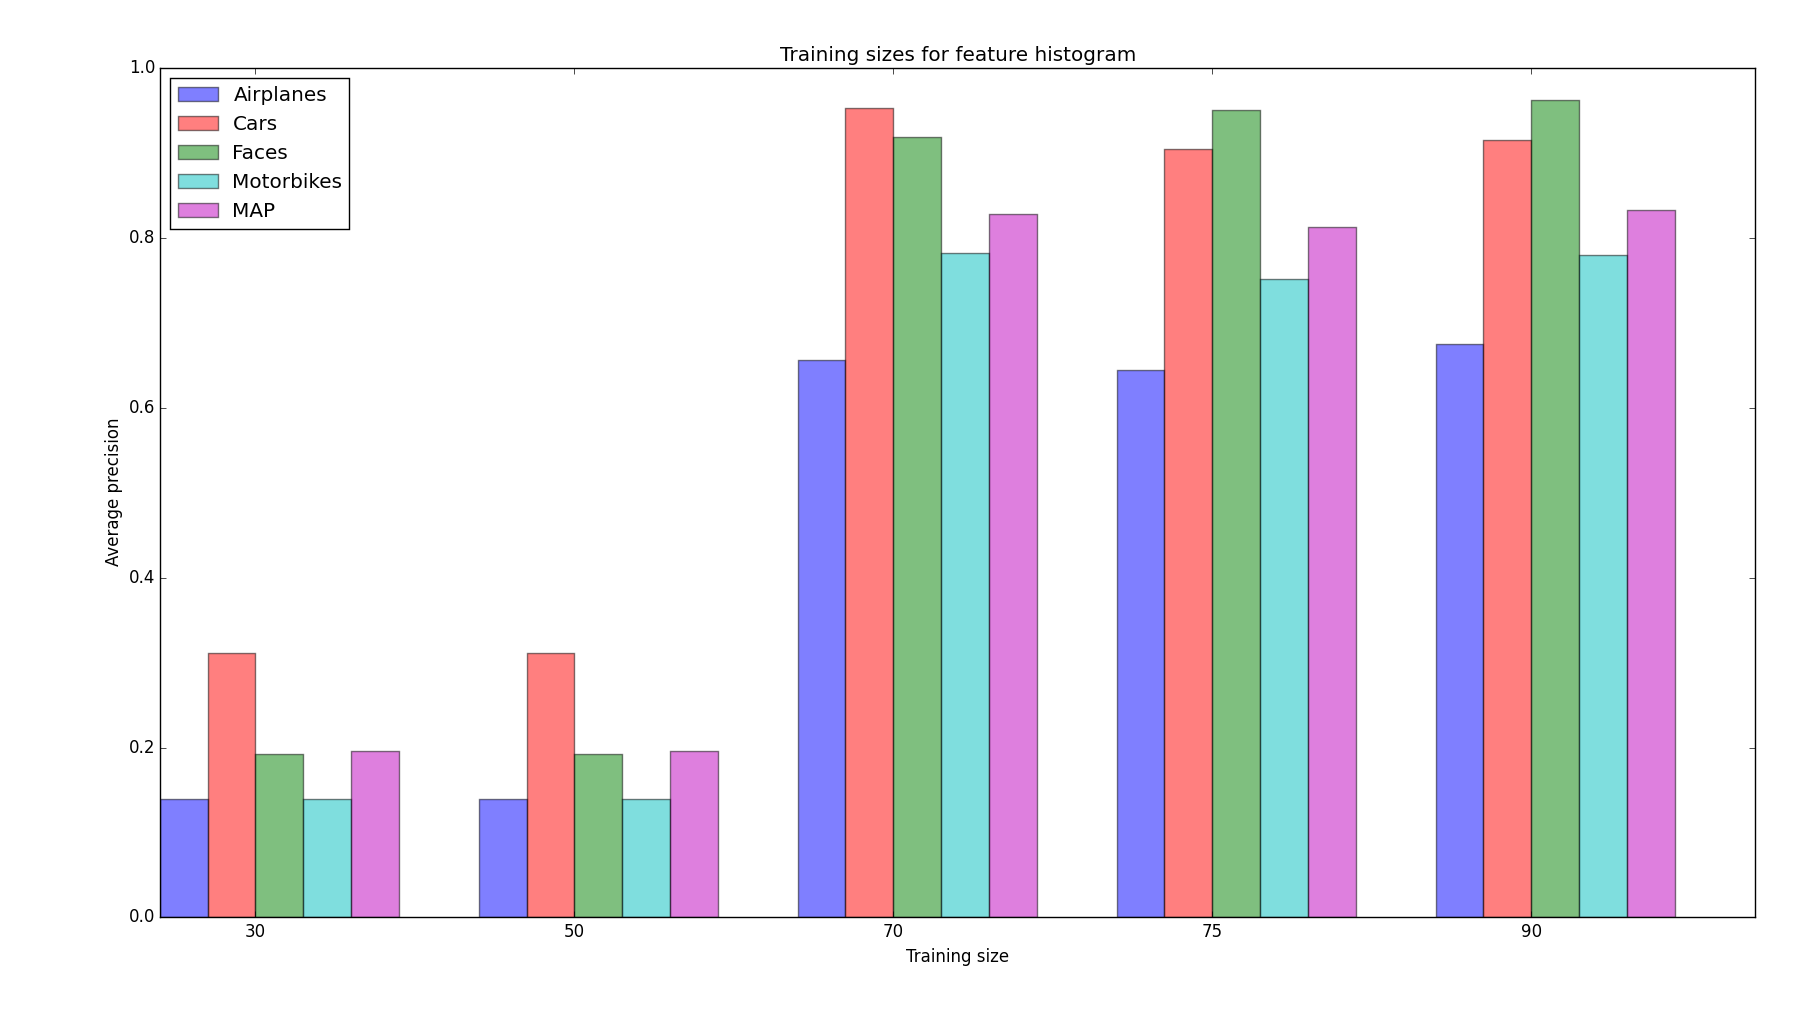
\includegraphics[scale=0.4]{plots/training_size_feature_histograms.png}
\caption{AP for different classes and MAP, for different training sizes for feature histogram}
\end{figure}

\begin{table}[H]
\begin{tabular}{|c|ccccc|}
\hline
\textbf{Training samples} & \textbf{AP Airplanes} & \textbf{AP Cars} & \textbf{AP Faces} & \textbf{AP Motorbikes} & \textbf{MAP}\\
\hline
30 & 0.1394 & 0.3118& 0.1924& 0.1394 & 0.1958\\
50 & 0.1394 & 0.3118& 0.1924& 0.1394 & 0.1958\\
70 & 0.6563 & 0.9534 & 0.9191 & 0.7830 & 0.8280\\
75 & 0.6447 & 0.9053 & 0.9510 & 0.7516 & 0.8132\\
90 & 0.6749 & 0.9157 & 0.9631 & 0.7798 & 0.8334\\
\hline
\end{tabular}
\caption{Effect number of training samples (per class) for feature histogram, Sift type: dense, Color space: opponent}
\end{table}


\subsection{Effect number of training samples for SVM}

\begin{table}[H]
\begin{tabular}{|c|ccccc|}
\hline
\textbf{Training samples} & \textbf{AP Airplanes} & \textbf{AP Cars} & \textbf{AP Faces} & \textbf{AP Motorbikes} & \textbf{MAP}\\
\hline
30 & 0.6647 & 0.8898 & 0.3772 & 0.5184& 0.6125\\
50 & 0.6484 & 0.9096 & 0.8780 & 0.6627 & 0.7747\\
70 & & & & & \\
75 & 0.6447 & 0.9053 & 0.9510 & 0.7516 & 0.8132\\
90 & & & & & \\
\hline
\end{tabular}
\caption{Effect number of training samples (per class) for SVM, Sift type: dense, Color space: opponent}
\end{table}


\subsection{Effect of different cluster sizes}

\begin{table}[H]
\begin{tabular}{|c|ccccc|}
\hline
\textbf{Cluster size} & \textbf{AP Airplanes} & \textbf{AP Cars} & \textbf{AP Faces} & \textbf{AP Motorbikes} & \textbf{MAP}\\
\hline
400 & 0.6447 & 0.9053 & 0.9510 & 0.7516 & 0.8132\\
800 & 0.6424 & 0.5067 & 0.9602 & 0.5667 & 0.6690\\
1600 & 0.6438 & 0.3115 & 0.8410 & 0.5361 & 0.5831 \\
2000 & 0.6367 & 0.7253 & 0.3357 & 0.1926 & 0.4726\\
4000 & & & & & \\
\hline
\end{tabular}
\caption{Effect of different cluster sizes, Sift type: dense, Color space: opponent}
\end{table}

\subsection{Effect of different step sizes for dense}

\begin{table}[H]
\begin{tabular}{|c|ccccc|}
\hline
\textbf{Step size} & \textbf{AP Airplanes} & \textbf{AP Cars} & \textbf{AP Faces} & \textbf{AP Motorbikes} & \textbf{MAP}\\
\hline
10 & 0.6823 & 0.8654 & 0.9444 & 0.6934 & 0.7964\\
20 & 0.6447 & 0.9053 & 0.9510 & 0.7516 & 0.8132\\
30 & & & & & \\
50 & & & & & \\
\hline
\end{tabular}
\caption{Effect of different step sizes for dense, Sift type: dense, Color space: opponent}
\end{table}


\subsection{Effect different kernels for SVM}

\begin{table}[H]
\begin{tabular}{|c|ccccc|}
\hline
\textbf{Kernel} & \textbf{AP Airplanes} & \textbf{AP Cars} & \textbf{AP Faces} & \textbf{AP Motorbikes} & \textbf{MAP}\\
\hline
sigmoid & 0.6447 & 0.9053 & 0.9510 & 0.7516 & 0.8132\\
linear & & & & & \\
polynomial & & & & & \\
radial & & & & & \\
\hline
\end{tabular}
\caption{Effect different kernels for SVM, Sift type: dense, Color space: opponent}
\end{table}
